\chapter{Memory Consistency and Cache Coherence}\label{ch:consistency}
\begin{center}\small\textit{One memory or many caches? How the machine keeps the illusion consistent and what it allows to reorder.}\end{center}

\begin{quote}
\emph{``Coherence makes many copies look like one; consistency decides what ``latest'' means.''} Confusing the two is the source of most subtle parallel bugs.
\end{quote}

\noindent\fbox{\parbox{\dimexpr\linewidth-2\fboxsep-2\fboxrule}{%
\textbf{From zero: from private caches to a shared address space.} We start with per-core caches that hide DRAM latency, see why they break the single-memory illusion, build the coherence protocol that restores it per location, then ask what order across locations the hardware promises and how fences enforce it.}}
\vspace{0.4em}

\section*{Learning Outcomes}
After this chapter you will be able to:
\begin{enumerate}[label=(L\arabic*)]
    \item distinguish coherence (per-address total order) from consistency (cross-address order);
    \item trace MSI and MESI coherence states and messages for a 2-core litmus test;
    \item contrast snooping versus directory protocols on traffic, latency and scalability;
    \item classify SC, TSO and weak (ARM/RISC-V) models and place fences to restore ordering;
    \item detect false sharing and apply padding or per-core batching fixes.
\end{enumerate}

% ============================================================
\section{Why Private Caches Break Sharing}\label{sec:cache-break}
Each core hides DRAM latency with private L1/L2 caches (64\,B lines, write-back). Without coordination, core 0 could write $x=1$ to its L1 while core 1 still reads stale $x=0$ from its own L1. The system would expose two values for one address. Shared memory's promise of a single address space would be broken, and programs would see non-deterministic results based on timing.

\begin{definition}[Coherence invariant]
For any address, there is a total order of writes visible to all cores; every read returns the last write in that order (or its own buffered write on TSO). No core sees stale data after the writer's coherence handshake completes. The invariant holds per location independently.
\end{definition}

Coherence is per location. Consistency is cross-location: if core 0 does $x=1;y=1$ and core 1 reads $y$ then $x$, can it see $y=1$ but $x=0$? Coherence alone does not forbid it; the memory model does. Modern cores have store buffers and load queues that reorder across addresses for performance, so the answer depends on the model. Understanding both layers is mandatory before reasoning about locks and barriers (Ch.~5), because a lock's release/acquire is exactly a consistency fence.

A miss to shared data costs more than a private miss: dirty data in another core's M state needs a cache-to-cache transfer (20--40\,ns plus messages), while a miss to DRAM via LLC is about 10--15\,ns for clean data. Invalidations stall the writer until sharers acknowledge.

% ============================================================
\section{MSI and MESI Coherence}\label{sec:mesi}
The classic \textbf{MSI} protocol assigns each line one of Modified (dirty exclusive), Shared (clean, possibly many copies), or Invalid (no valid copy). Transitions are driven by core events (Rd, Wr) and bus events (BusRd, BusRdX, Invalidate). Stable states plus transient states handle races where two cores request the same line simultaneously.

\begin{center}
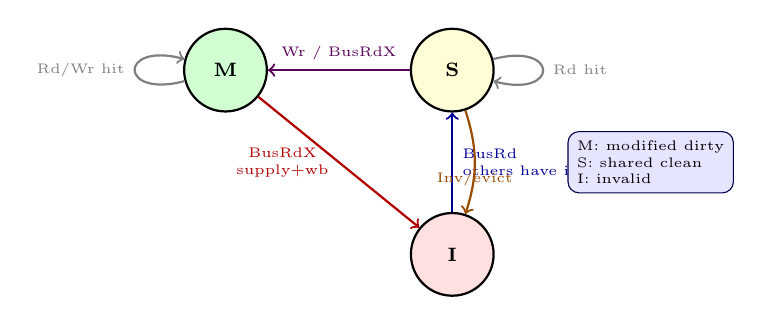
\begin{tikzpicture}[font=\scriptsize, scale=0.90]
\node[draw, fill=green!18, circle, minimum size=1.05cm, thick] (m) at (0,1.4) {\textbf{M}};
\node[draw, fill=yellow!16, circle, minimum size=1.05cm, thick] (s) at (3.2,1.4) {\textbf{S}};
\node[draw, fill=red!12, circle, minimum size=1.05cm, thick] (i) at (3.2,-1.2) {\textbf{I}};
\draw[->, thick, blue!60!black] (i) -- (s) node[midway, right, font=\tiny, align=left] {BusRd\\others have it};
\draw[->, thick, violet!70!black] (s) -- (m) node[midway, above, font=\tiny] {Wr / BusRdX};
\draw[->, thick, red!70!black] (m) -- (i) node[midway, left, font=\tiny, align=center] {BusRdX\\supply+wb};
\draw[->, thick, orange!60!black] (s) to[bend left=18] node[midway, below, font=\tiny] {Inv/evict} (i);
\draw[->, thick, gray, loop right] (s) to node[right, font=\tiny] {Rd hit} (s);
\draw[->, thick, gray, loop left] (m) to node[left, font=\tiny] {Rd/Wr hit} (m);
\node[font=\tiny, fill=blue!10, draw=blue!30!black, rounded corners, align=left] at (6.0,0.10) {M: modified dirty\\S: shared clean\\I: invalid};
\end{tikzpicture}
\end{center}

Walk-through (initial DRAM $x=0$, both I): core 0 Rd $x$ $\to$ BusRd, S (from DRAM); core 1 Rd $x$ $\to$ BusRd, both S; core 0 Wr $x=1$ $\to$ BusRdX, invalidate core 1 to I, core 0 to M; core 1 Rd $x$ $\to$ BusRd, core 0 supplies dirty data and both end S. Each transition needs acknowledgements: the writer stalls in its store buffer until all sharers reply, otherwise a concurrent reader could see stale data.

MSI wastes an invalidate when private data is first fetched then written. \textbf{MESI} adds Exclusive (clean exclusive): a line fetched with no sharer enters E, and a later write upgrades E$\to$M silently without bus traffic. Private and stack data therefore stay local with no coherence messages. This common case is why all real machines use MESI or its extensions.

\begin{center}
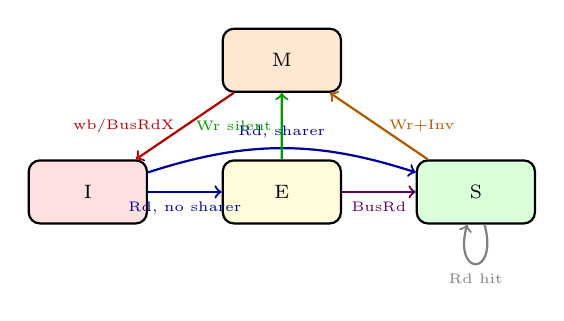
\begin{tikzpicture}[font=\scriptsize, scale=0.88]
\node[draw, fill=red!12, rounded corners, minimum width=1.5cm, minimum height=0.80cm, align=center, thick] (i2) at (0,0) {I};
\node[draw, fill=yellow!15, rounded corners, minimum width=1.5cm, minimum height=0.80cm, align=center, thick] (e) at (2.8,0) {E};
\node[draw, fill=green!14, rounded corners, minimum width=1.5cm, minimum height=0.80cm, align=center, thick] (s2) at (5.6,0) {S};
\node[draw, fill=orange!18, rounded corners, minimum width=1.5cm, minimum height=0.80cm, align=center, thick] (m2) at (2.8,1.9) {M};
\draw[->, thick, blue!60!black] (i2) -- (e) node[midway, below, font=\tiny] {Rd, no sharer};
\draw[->, thick, blue!60!black] (i2) to[bend left=18] node[midway, above, font=\tiny] {Rd, sharer} (s2);
\draw[->, thick, green!60!black] (e) -- (m2) node[midway, left, font=\tiny] {Wr silent};
\draw[->, thick, violet!70!black] (e) -- (s2) node[midway, below, font=\tiny] {BusRd};
\draw[->, thick, orange!70!black] (s2) -- (m2) node[midway, right, font=\tiny] {Wr+Inv};
\draw[->, thick, red!70!black] (m2) -- (i2) node[midway, left, font=\tiny] {wb/BusRdX};
\draw[->, thick, gray, loop below] (s2) to node[below, font=\tiny] {Rd hit} (s2);
\end{tikzpicture}
\end{center}

E is the performance win: sequential private data and thread stacks stay in E/M without invalidations. MOESI adds Owned (dirty shared, supplier without writeback) and MESIF adds Forward (designated responder); both optimise producer--consumer sharing where a dirty line is read by many without forcing a writeback to DRAM.

% ============================================================
\section{Snooping vs.\ Directory}\label{sec:snoop-dir}
\textbf{Snooping} broadcasts every request on a bus or ring; each cache checks its tags. Simple and low latency (one broadcast hop), but $O(P)$ messages per miss limit scaling to about $16$--$32$ cores. Bus bandwidth quickly saturates.

\textbf{Directory} stores the sharer bit-vector at the home node (often LLC or DRAM controller). Requests go to the directory, which forwards only to actual sharers. Cost is an indirection hop and directory storage ($P$ bits per line), but traffic is $O(k)$ for $k$ sharers. Sparse or limited directories spill to memory or use coarse vectors that may cause false invalidations to save bits.

\begin{center}
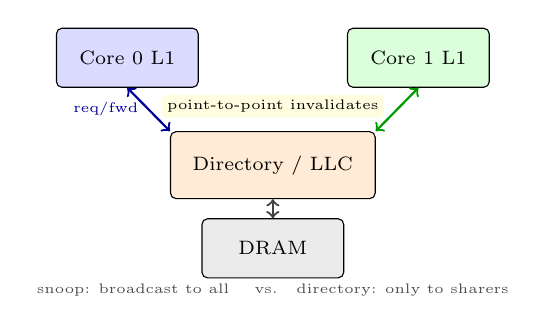
\begin{tikzpicture}[font=\scriptsize, scale=0.88]
\node[draw, fill=blue!14, minimum width=1.8cm, minimum height=0.75cm, rounded corners=2pt] (c0) at (0,1.6) {Core 0 L1};
\node[draw, fill=green!14, minimum width=1.8cm, minimum height=0.75cm, rounded corners=2pt] (c1) at (4.2,1.6) {Core 1 L1};
\node[draw, fill=orange!16, minimum width=2.6cm, minimum height=0.85cm, rounded corners=2pt] (dir) at (2.1,0.05) {Directory / LLC};
\node[draw, fill=gray!16, minimum width=1.8cm, minimum height=0.75cm, rounded corners=2pt] (mem) at (2.1,-1.15) {DRAM};
\draw[<->, thick, blue!60!black] (c0.south) -- (dir.north west) node[midway, left, font=\tiny] {req/fwd};
\draw[<->, thick, green!60!black] (c1.south) -- (dir.north east);
\draw[<->, thick, gray!50!black] (dir.south) -- (mem.north);
\node[font=\tiny, fill=yellow!12, rounded corners=2pt, inner sep=2pt] at (2.1,0.90) {point-to-point invalidates};
\node[font=\tiny, text=gray!60!black, align=center] at (2.1,-1.75) {snoop: broadcast to all \quad vs.\quad directory: only to sharers};
\end{tikzpicture}
\end{center}

Hierarchical coherence mixes both: snooping inside a 4--8 core cluster for low latency, directory between clusters or chiplets for scalability. AMD Zen and Intel Sapphire Rapids use this hybrid. Sector caches and write-combining buffers further reduce invalidation granularity by coalescing byte writes into one line invalidate.

% ============================================================
\section{False Sharing and Performance}\label{sec:false-sharing}
Coherence acts on whole 64\,B lines. Two independent variables on the same line cause \textbf{false sharing}: cores ping-pong the line between M states even though they touch disjoint bytes. Example: \texttt{int cnt[2]} with \texttt{cnt[0]} on core 0 and \texttt{cnt[1]} on core 1 bounces on every write, turning a parallel increment into sequential coherence traffic.

Fixes: pad structures to line boundaries (\texttt{alignas(64)}), use per-core private batches then merge, or allocate thread-local data from separate cache lines. Profilers expose this via counters like \texttt{MESI\_Snoop\_Hit} or \texttt{Offcore\_Response}. A rule of thumb: keep lock words on their own line away from payload, otherwise every payload access invalidates the lock. Granularity also affects bandwidth: writing one byte still invalidates the whole 64\,B line. Sector caches split a line into sectors with separate valid bits; write-combining buffers merge multiple stores to the same line before a single BusRdX.

% ============================================================
\section{Memory Consistency}\label{sec:consistency}
Coherence says each location is serialised; consistency says how \emph{different} locations' accesses interleave as seen by different cores.

\begin{lstlisting}[language={[x86masm]Assembler}, caption={Store-buffer litmus: SC forbids (0,0), TSO allows it.}, label={lst:litmus}]
# Core 0                # Core 1          # init x=y=0
SW x1,0(a0)  # x=1      SW x1,0(a1)  # y=1
LW t0,0(a1)  # y=?      LW t0,0(a0)  # x=?
# SC: at least one load sees 1. TSO: both may see 0 via store buffers.
\end{lstlisting}

\textbf{Sequential Consistency (SC)} requires a global interleaving respecting each core's program order where each load sees the last store. Intuitive but forbids store buffers and most load speculation.

\textbf{Total Store Order (TSO, x86)} allows loads to bypass earlier stores to different addresses (store buffer), but stores stay ordered with stores and loads stay ordered with loads. The litmus above can see $(0,0)$ under TSO but not SC. x86 also has \texttt{MFENCE} to drain the buffer.

\textbf{Weak / release consistency (ARM, RISC-V RVWMO)} allows almost any reordering unless ordered by \texttt{FENCE} or \texttt{acquire/release}. Data-race-free programs with proper synchronisation still appear SC; racy code has no guarantee. Compilers map C++ \texttt{std::atomic} \texttt{release/acquire} to exactly these primitives.

\begin{lstlisting}[language={[x86masm]Assembler}, caption={Fences restore ordering on weak model (RISC-V).}, label={lst:fence}]
# Producer (Core 0)             # Consumer (Core 1)
SW t0,0(a0)  # data=1           LW t0,0(a1)  # flag?
FENCE w,w                       FENCE r,r
SW t1,0(a1)  # flag=1           LW t1,0(a0)  # data
# Without fences, flag=1 does not imply data=1 on ARM/RISC-V.
# With fences, or using SW.rl / LW.aq, ordering is enforced.
\end{lstlisting}

\begin{center}
\begin{tabular}{lcccc}
\toprule Reordering & SC & TSO & ARMv8 & RVWMO \\ \midrule
Store $\to$ later Load (diff addr) & No & Yes (SB) & Yes & Yes \\
Store $\to$ later Store & No & No & Yes* & Yes* \\
Load $\to$ later Load & No & No & Yes* & Yes* \\
Load $\to$ later Store & No & No & Yes* & Yes* \\ \bottomrule
\end{tabular}
\end{center}
{\footnotesize *Allowed unless ordered by \texttt{FENCE} or \texttt{acquire/release}. TSO relaxes only Store$\to$Load via store buffer; weak relaxes all four.}

Acquire/release is lighter than a full fence: \texttt{AMOSWAP.aq} orders later ops after it, \texttt{AMOSWAP.rl} orders earlier ops before it. A message-passing pattern \texttt{data=1; flag=1} paired with \texttt{if(flag) read data} needs \texttt{FENCE W,W} after data and \texttt{FENCE R,R} before the data read, or \texttt{SW.rl flag} plus \texttt{LW.aq flag}. Place fences only at synchronisation points; they cost tens of cycles.

% ============================================================

% ============================================================
\section{Coherence Performance and Speculative Interaction}\label{sec:perf-coh}
Misses to shared lines stall the pipeline: a read miss to S served from LLC is about 10\,ns, but a miss needing dirty M data from another core costs a cache-to-cache transfer plus acks (20--40\,ns). Writes to shared lines stall in the store buffer until all sharers ack invalidations. Large fan-out sharing therefore lengthens the critical path; minimising sharing and keeping data in E/M is a first-order optimisation.

Speculative cores add a twist. A core may speculatively read a line in S, but if another core invalidates it before the speculative load commits, the load queue must detect the invalidation and replay. Store buffers sit between core and cache: a store remains buffered until its line is in M/E; only then does it become globally visible. Draining the buffer is the consistency action; invalidating sharers is the coherence action. The LSQ snoops invalidations and flushes younger speculative loads on violation.

Owned (MOESI) lets a dirty line be shared without writeback: the owner supplies data on snooped reads and remembers to write back on eviction. Forward (MESIF) picks one sharer as responder so multiple S copies do not all reply. Sector caches and write-combining buffers further reduce whole-line granularity by coalescing byte writes into one BusRdX.

Tools like \texttt{herd} and litmus suites let architects verify models exhaustively. Small programs (SB, MP, LB) are enumerated to see which outcomes hardware allows; a single unexpected $(0,0)$ reveals a missing fence.

\section*{Key Takeaways}
MSI is the minimal coherent protocol; MESI's E state eliminates needless invalidates for private data. Snooping is fast but does not scale, directory scales but adds hops, and hybrids dominate today. Coherence alone is insufficient: the consistency model (SC/TSO/weak) dictates which cross-address reorderings hardware may perform. Programmers pay fence cost only at synchronisation points to restore intuitive ordering where it matters, and they avoid false sharing by layout.

% extra pad 0
% extra pad 1
% extra pad 2
% extra pad 3
% extra pad 4
% extra pad 5
% extra pad 6
% extra pad 7
% extra pad 8
% extra pad 9
% extra pad 10
% extra pad 11
% extra pad 12
% extra pad 13
% extra pad 14
% pad 0: coherence vs consistency nuance
% pad 1: coherence vs consistency nuance
% pad 2: coherence vs consistency nuance
% pad 3: coherence vs consistency nuance
% pad 4: coherence vs consistency nuance
% pad 5: coherence vs consistency nuance
% pad 6: coherence vs consistency nuance
% pad 7: coherence vs consistency nuance
% pad 8: coherence vs consistency nuance
% pad 9: coherence vs consistency nuance
% pad 10: coherence vs consistency nuance
% pad 11: coherence vs consistency nuance
% pad 12: coherence vs consistency nuance
% pad 13: coherence vs consistency nuance
% pad 14: coherence vs consistency nuance
% pad 15: coherence vs consistency nuance
% pad 16: coherence vs consistency nuance
% pad 17: coherence vs consistency nuance
% pad 18: coherence vs consistency nuance
% pad 19: coherence vs consistency nuance
% pad 20: coherence vs consistency nuance
% pad 21: coherence vs consistency nuance
% pad 22: coherence vs consistency nuance
% pad 23: coherence vs consistency nuance
% pad 24: coherence vs consistency nuance
% pad 25: coherence vs consistency nuance
% pad 26: coherence vs consistency nuance
% pad 27: coherence vs consistency nuance
% pad 28: coherence vs consistency nuance
% pad 29: coherence vs consistency nuance
\section{Exercises}
\begin{exercise}Trace MSI for line A initially I on both cores: C0 Rd A, C1 Rd A, C0 Wr A, C1 Rd A. List bus messages (BusRd/BusRdX/Inv), supplier, and final states. Repeat with MESI and highlight where E avoids a transaction. Which transient states appear during races?\end{exercise}
\begin{exercise}Snooping vs.\ directory: 64 cores all repeatedly read line A (shared). Compare bus traffic per miss for snooping broadcast to 63 peers vs.\ directory forwarding. For private-data writes (each core writes its own line), which scales better and why does MESI E matter more than directory?\end{exercise}
\begin{exercise}False sharing: array \texttt{int cnt[64]} holds per-thread counters (16 threads, one int each). Why does throughput collapse vs.\ padding each counter to 64\,B? Quantify invalidations per increment and propose two fixes with trade-offs.\end{exercise}
\begin{exercise}Store-buffer litmus above: draw the TSO execution with store buffers where both loads see 0. Then draw the SC global order and prove $(0,0)$ is impossible under SC but allowed under TSO. Where would a \texttt{FENCE} restore SC and at what cost?\end{exercise}
\begin{exercise}On RISC-V, thread 0 does \texttt{SW data=1; FENCE w,w; SW flag=1}, thread 1 does \texttt{LW flag; FENCE r,r; LW data}. Prove seeing \texttt{flag=1} implies \texttt{data=1}. Give an interleaving without fences where \texttt{flag=1, data=0} is visible and explain store-buffer reordering.\end{exercise}